\section{AG 2.1 - 1 Aequivalenz von Formeln - MC - BIFIE}

\begin{beispiel}[AG 2.1]{1} %PUNKTE DES BEISPIELS
Die nachstehende Abbildung zeigt ein Trapez. 

\begin{center}
\definecolor{zzttqq}{rgb}{0.266666666667,0.266666666667,0.266666666667}
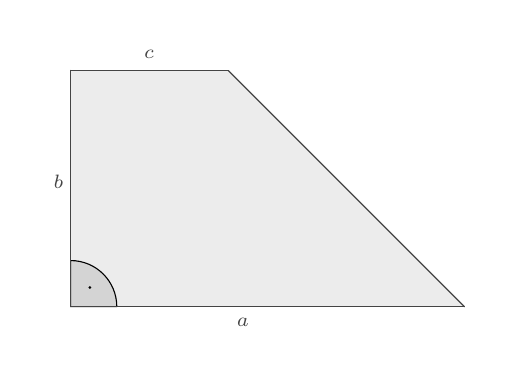
\begin{tikzpicture}[line cap=round,line join=round,x=1.0cm,y=1.0cm]
\clip(1.45375609756,2.52351219512) rectangle (7.22936585366,6.54302439024);
\fill[color=zzttqq,fill=zzttqq,fill opacity=0.1] (2.,6.) -- (4.,6.) -- (7.,3.) -- (2.,3.) -- cycle;
\draw [shift={(2.,3.)},fill=black,fill opacity=0.1] (0,0) -- (0.:0.585365853659) arc (0.:90.:0.585365853659) -- cycle;
\draw [color=zzttqq] (2.,6.)-- (4.,6.);
\draw [color=zzttqq] (4.,6.)-- (7.,3.);
\draw [color=zzttqq] (7.,3.)-- (2.,3.);
\draw [color=zzttqq] (2.,3.)-- (2.,6.);
\fill[fill=black,fill opacity=1] (2.24348009682,3.24348009682) circle (0.019512195122);
\begin{scriptsize}
\draw[color=zzttqq] (2.9952195122,6.2) node {$c$};
\draw[color=zzttqq] (4.18546341463,2.8) node {$a$};
\draw[color=zzttqq] (1.844,4.59180487805) node {$b$};
\end{scriptsize}
\end{tikzpicture}
\end{center}

Mit welchen der nachstehenden Formeln kann man die Fl�che dieses Trapezes berechnen?

Kreuze die zutreffende(n) Formel(n) an!

\multiplechoice[5]{  %Anzahl der Antwortmoeglichkeiten, Standard: 5
				L1={$A_1=\frac{1}{2}\cdot (a+c)\cdot b$},   %1. Antwortmoeglichkeit 
				L2={$A_2=b\cdot c + \frac{(a-c)\cdot b}{2}$},   %2. Antwortmoeglichkeit
				L3={$A_3=a\cdot b - 0,5 \cdot (a-c)\cdot b$},   %3. Antwortmoeglichkeit
				L4={$A_4=0,5\cdot a \cdot b - (a+c)\cdot b$},   %4. Antwortmoeglichkeit
				L5={$A_5=\frac{1}{2}\cdot a \cdot b + b \cdot c$},	 %5. Antwortmoeglichkeit
				L6={},	 %6. Antwortmoeglichkeit
				L7={},	 %7. Antwortmoeglichkeit
				L8={},	 %8. Antwortmoeglichkeit
				L9={},	 %9. Antwortmoeglichkeit
				%% LOESUNG: %%
				A1=1,  % 1. Antwort
				A2=2,	 % 2. Antwort
				A3=3,  % 3. Antwort
				A4=0,  % 4. Antwort
				A5=0,  % 5. Antwort
				}


\end{beispiel}